\section{Software Design}
{\tinyWritten by: Sven}

\subsection{Introduction}

This chapter delves into the intricate details of the software design employed in the
development of the locker system for university environments. A robust and efficient
software architecture is pivotal in ensuring the seamless functioning and user satisfaction
of the system. In this section, we provide an overview of the architectural approach,
technologies, and frameworks chosen for the implementation of the locker system software,
highlighting their significance and relevance to the project objectives.

\begin{figure}[h]
    \centering
    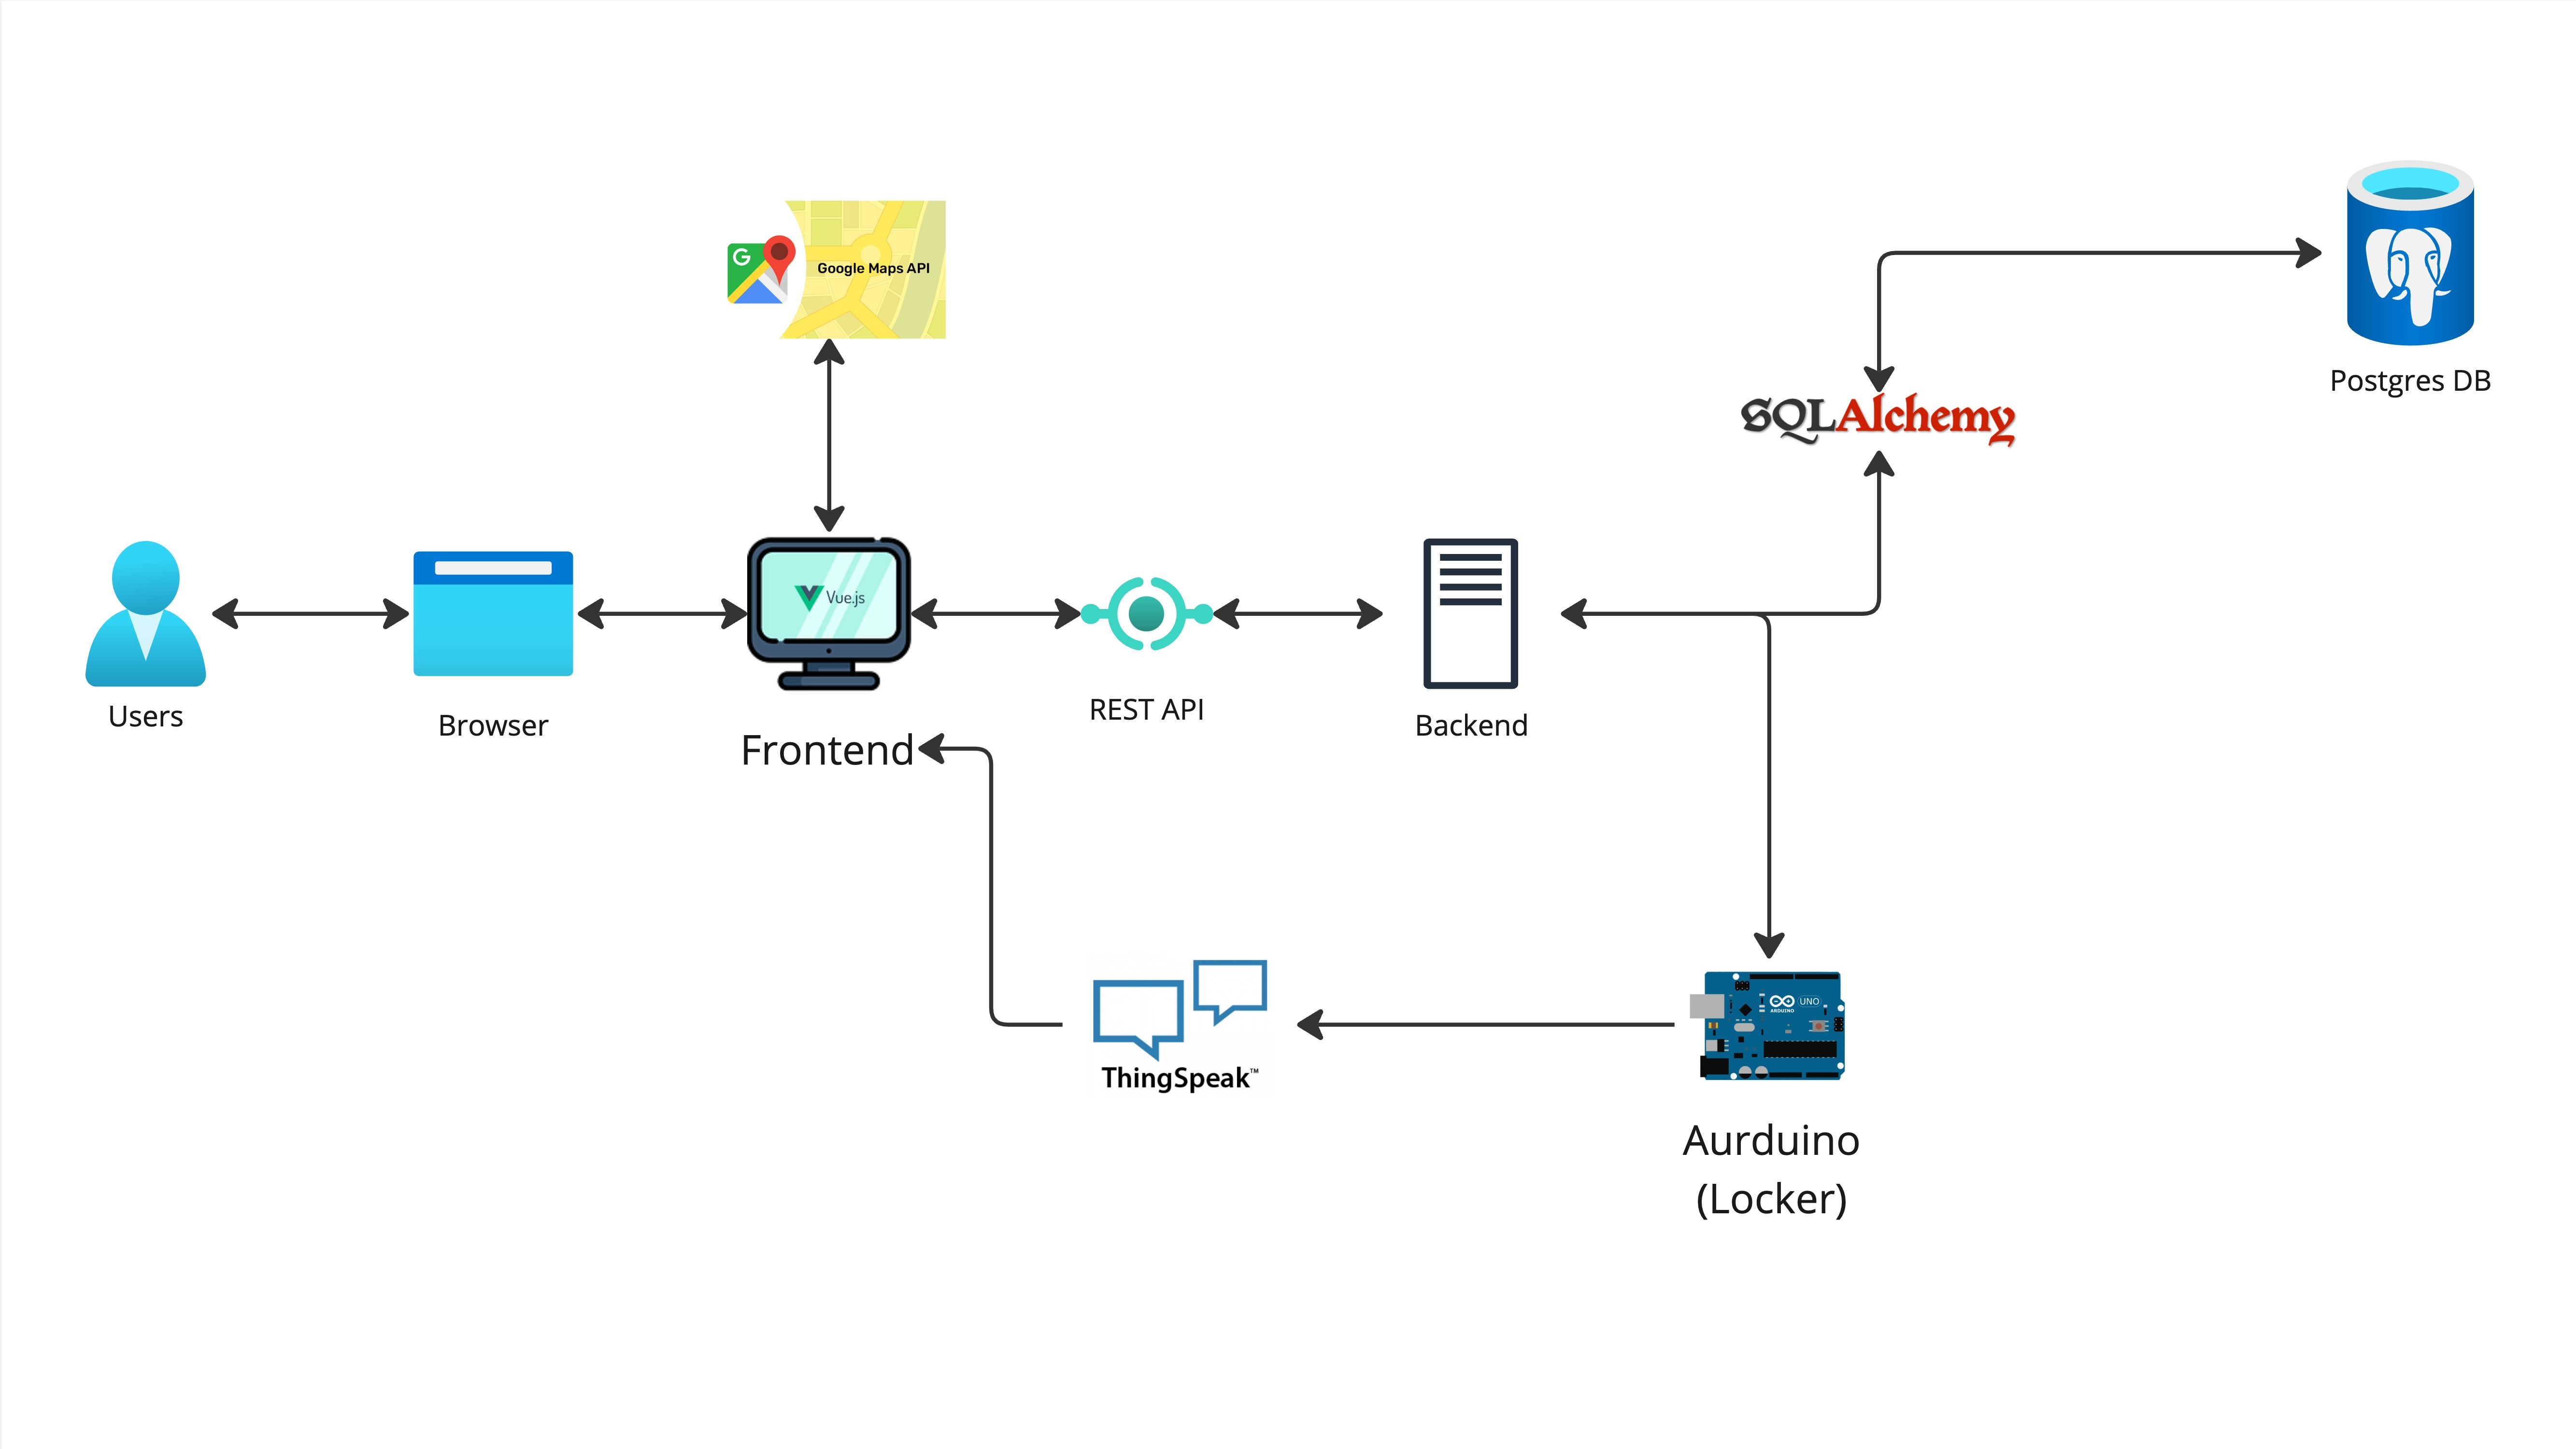
\includegraphics[width=0.8\textwidth]{images/software_design_diagram}
    \caption{Software Design Diagram}
    \label{fig:software_design}
\end{figure}

The image above depicts a high-level overview of the software design architecture,
illustrating the interaction between various components and their roles within the system.
Throughout this chapter, we elucidate the rationale behind each architectural decision
and technology selection, elucidating their benefits and contributions to the overall
functionality and performance of the locker system.

Now, let's delve into the intricacies of the software design, beginning with an exploration
of the architectural approach adopted for the project.


\subsection{Architectural Approach}

The adoption of a modern microservices architecture, with clear separation between
frontend and backend components, offers several advantages for the locker system project.
By decoupling these layers and enabling communication via a RESTful API, we achieve enhanced
modularity, scalability, and flexibility. This modular approach facilitates
independent development and deployment of frontend and backend services, enabling
rapid iteration and evolution of the system. Moreover, the RESTful API design simplifies
integration with third-party services and future expansion of functionality, ensuring
adaptability to changing requirements and technological advancements.

\subsection{Frontend Technologies}

Vue.js was selected as the frontend framework due to its lightweight nature, simplicity,
and extensive ecosystem of plugins and libraries. Its reactive data binding and component-based
architecture enable the creation of dynamic and interactive user interfaces, enhancing
the user experience. Additionally, the integration of Tailwind CSS and Bootstrap provides
a comprehensive set of styling utilities and pre-designed components, enabling rapid
prototyping and ensuring consistent design across different devices and screen sizes.
The use of these frontend technologies not only accelerates development but also enhances
maintainability and scalability, making them well-suited for a complex application like
the locker system.

\subsection{Google Maps Integration}

The integration of the Google Maps API enriches the user experience by providing visual
representation of locker locations. This feature enhances user convenience and navigation,
particularly in large university campuses where locker locations may not be readily apparent.
By leveraging the Google Maps API, users can easily locate their rented devices, thereby
reducing frustration and improving overall satisfaction with the service.

\subsection{Backend Technologies}

FastAPI was chosen as the backend framework due to its high performance,
asynchronous capabilities, and intuitive API design. Its built-in support for
asynchronous programming enables efficient handling of concurrent requests,
ensuring optimal responsiveness and scalability, especially under heavy loads.
Additionally, FastAPI's automatic generation of OpenAPI documentation simplifies
API documentation and client integration, enhancing developer productivity and collaboration.
The use of FastAPI aligns with industry best practices and standards, ensuring the reliability,
security, and maintainability of the locker system backend.

\subsection{Database Management}

The utilization of SQLAlchemy as the ORM tool offers numerous benefits for database management
within the locker system project. By abstracting away the complexities of database interaction,
SQLAlchemy enhances developer productivity and code maintainability,
while also mitigating the risk of SQL injection vulnerabilities. Furthermore,
Alembic provides seamless database schema versioning and migration capabilities,
facilitating continuous evolution and refinement of the database schema over time.
These features ensure data integrity, consistency, and scalability, making SQLAlchemy
and Alembic well-suited for managing the relational database backend of the locker system.

\subsection{Database Choice}

PostgreSQL was selected as the underlying database management system for its robustness,
reliability, and advanced feature set. Its support for ACID transactions,
data integrity constraints, and extensible data types ensures the consistency and
integrity of stored data, critical for a mission-critical application like the locker system.
Additionally, PostgreSQL's scalability and performance optimizations make it capable
of handling large volumes of concurrent transactions and complex queries, making it an ideal
choice for the storage and retrieval of locker rental and user data.

\subsection{Locker Controls}

The integration of Arduino-based locker controls provides a cost-effective and
customizable solution for managing locker access and device rentals. Arduino's open-source
hardware platform, coupled with its rich ecosystem of sensors and actuators, enables the
implementation of tailored locker control mechanisms suited to the specific requirements of
the locker system. By exposing REST APIs for communication with the backend, Arduino controllers
facilitate real-time updates and authentication checks, ensuring secure and reliable access to
rented devices.

\subsection{Charging Data Management}

ThingSpeak serves as an IoT analytics platform for collecting, storing, and visualizing
charging data generated by the Arduino controllers. Its cloud-based infrastructure and
user-friendly interface simplify data management and analysis, enabling administrators to
monitor charging activities and usage patterns in real-time. The integration of ThingSpeak
with the frontend enables the seamless transmission of processed data for visualization,
empowering administrators to make informed decisions regarding resource allocation and system
optimization.

\subsection{Hosting and Deployment}

The successful deployment and hosting of the locker system components are crucial for ensuring accessibility, scalability, and reliability. In this section, we elucidate the deployment strategies employed for the frontend, backend, and database components, leveraging cloud-based solutions and containerization technologies for seamless deployment and management.

\begin{figure}[h]
    \centering
    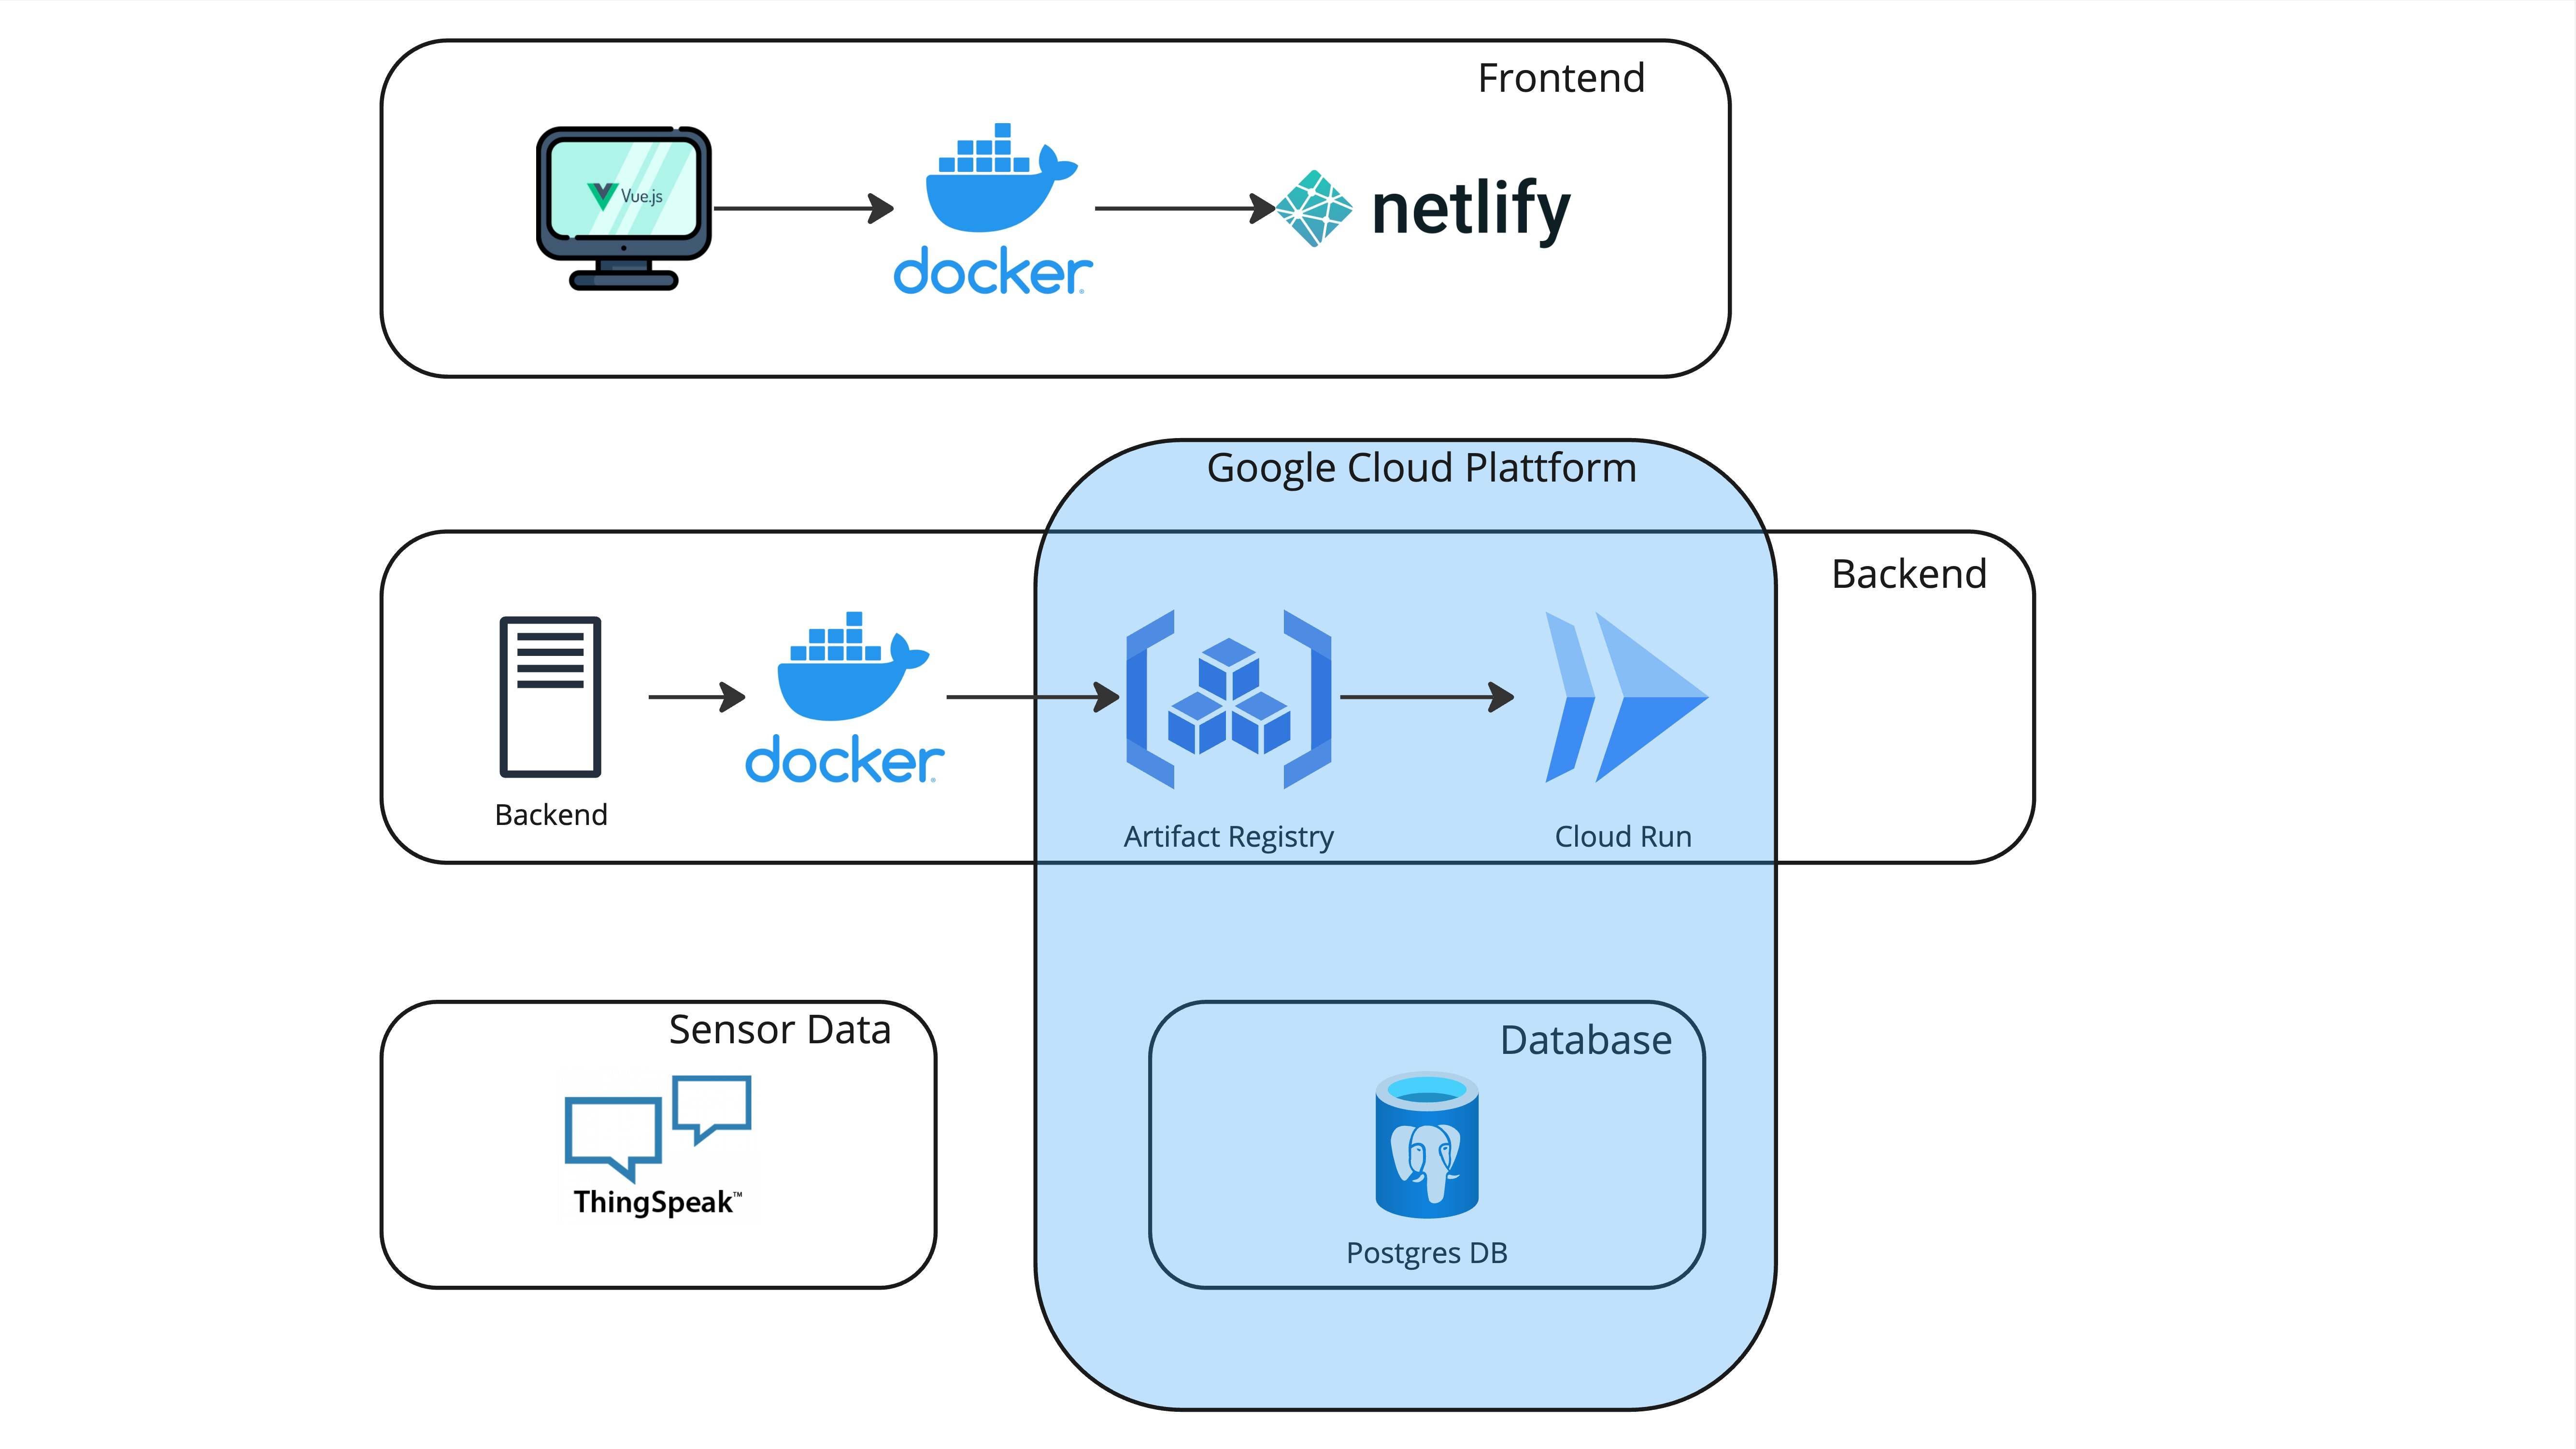
\includegraphics[width=0.8\textwidth]{images/software_design_deployment}
    \caption{Overview of Deployment Processes}
    \label{fig:deployment_overview}
\end{figure}

\subsubsection{Frontend Deployment}

The frontend of the locker system is packaged into a Docker container to encapsulate its dependencies and environment. This containerized approach ensures consistency and portability across different environments, mitigating potential compatibility issues. Subsequently, the Docker container is deployed to Netlify, a popular platform for hosting static websites and web applications. Netlify provides a straightforward deployment process, seamless integration with Git repositories, and automatic build and deployment pipelines. Additionally, Netlify assigns a public address to the deployed frontend, enabling users to access the locker system via the internet with ease.

\subsubsection{Backend Deployment}

Similar to the frontend, the backend services are containerized using Docker to streamline deployment and management. Once the backend Docker image is built, it is pushed to Google Cloud's Artifact Registry, a managed service for storing container images securely. Artifact Registry ensures version control, access control, and image vulnerability scanning, enhancing the security and reliability of the deployment process. Subsequently, the containerized backend services are deployed to Google Cloud Run, a fully managed serverless platform for running containerized applications. Google Cloud Run automatically scales the backend services based on demand, ensuring optimal performance and cost-efficiency. Furthermore, Google Cloud Run assigns a public address to the deployed backend services, facilitating seamless communication with the frontend and other system components over the internet.

\subsubsection{Database Hosting}

The PostgreSQL database used by the locker system is hosted on Google Cloud SQL, a fully managed relational database service. Google Cloud SQL offers automatic backups, high availability, and scalability, relieving the burden of database administration and maintenance. By leveraging Google Cloud SQL, we ensure data durability, reliability, and performance, critical for the storage and retrieval of locker rental and user data. Additionally, Google Cloud SQL provides seamless integration with other Google Cloud services, simplifying data management and access control.

\subsubsection{Sensor Data Management}

The sensor data collected by the Arduino controllers is transmitted to ThingSpeak, a cloud-based IoT analytics platform. ThingSpeak provides a scalable and reliable infrastructure for storing, analyzing, and visualizing sensor data in real-time. As a Software as a Service (SaaS) solution, ThingSpeak eliminates the need for hosting and infrastructure management, allowing developers to focus on application logic and data analysis. By leveraging ThingSpeak, we ensure efficient management and utilization of the sensor data.

\subsection{Conclusion}

In summary, the deployment and hosting of the locker system components leverage cloud-based solutions and containerization technologies to ensure accessibility, scalability, and reliability. By utilizing platforms such as Netlify, Google Cloud, and ThingSpeak, we streamline the deployment process, enhance security and performance, and enable seamless integration between different system components. This comprehensive approach to hosting and deployment underscores the importance of utilizing cloud-native technologies and services for building robust and scalable applications in modern computing environments.

The software design of the locker system incorporates a carefully selected set of technologies and architectural principles tailored to the specific requirements and challenges of managing locker rentals and device access in university environments. Many of these technologies were introduced in lectures at our university, and while there may be other options available, we opted for those recommended by the university and with which we had prior experience. By leveraging modern frameworks, platforms, and best practices, the system delivers enhanced functionality, scalability, and user experience, ensuring its effectiveness and viability in real-world deployments.

